\chapter{Results and Interpretation}

\section{Parameters and Nondimensionalization}

For most analyses, many of the parameters and results are non-dimensionalized. In
particular, instead of separate parameters for \(k_z\) and \(k_{xy}\), \(k_z\)
and \(k_{\textrm{meas}}\) are both normalized by \(k_{xy}\). Numerical
experiments verified that this is permissible, as numerical experiments with
different \(k_z\) and \(k_{xy}\) parameters but equivalent ratios
\(\fracflat{k_z}{k_{xy}}\) resulted in very similar ratios of
\(\fracflat{k_{\textrm{meas}}}{k_{xy}}\).

Angle is an exception. In this analysis, all angles are given as degrees from
the horizontal (\(xy\)) plane.

\section{Numerical vs. Analytical Predictions}

A 3-D plot of the numerical and analytical predictions may be seen in 
Figure \ref{fig:numvanal}.

\begin{figure}[h]
\centering
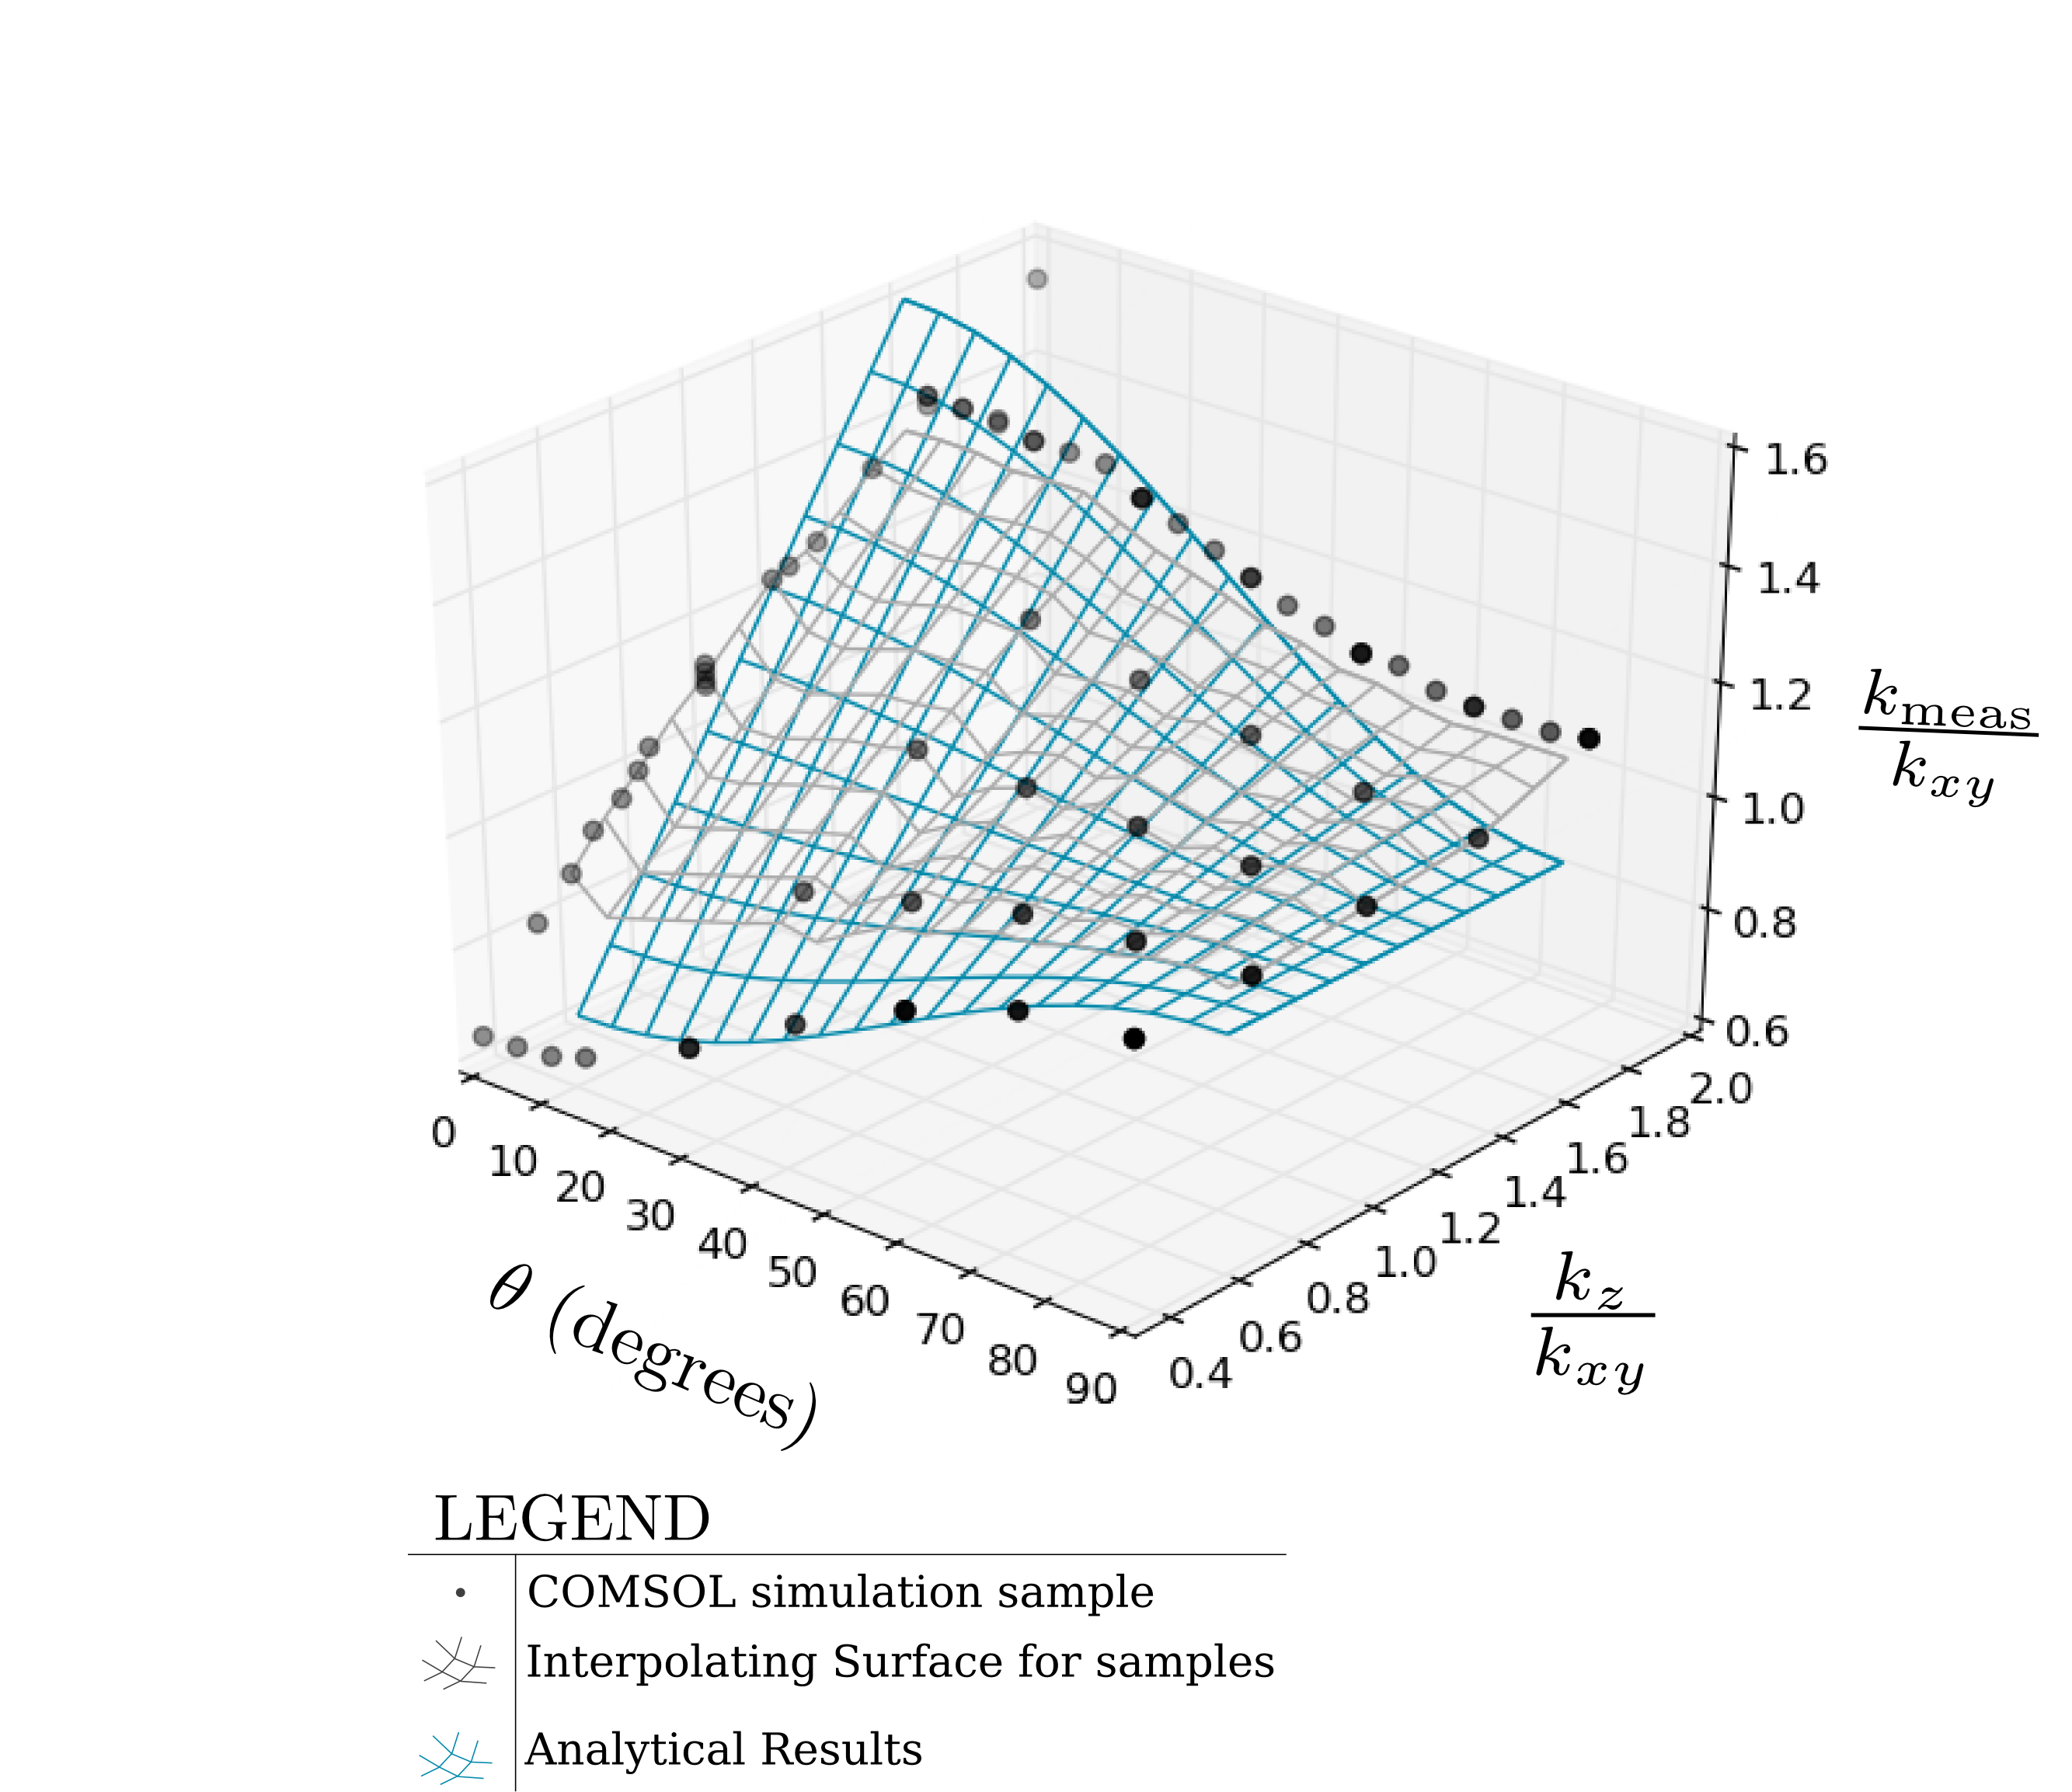
\includegraphics[width=\textwidth]{fig/numvanal.png}
\label{fig:numvanal}
\caption{A comparison of the numerical results and the analytical theory shows
general agreement. Grey dots represent numerical simulation results, the grey surface represents an interpolating surface of the dots, and the blue surface represents the analytical model. Disagreement between the two may be due to edge effects and/or numerical
model convergence issues.}
\end{figure}

This plot shows that the two approaches to predicting measured conductivity
as a function of angle and anisotropy ratio are in general agreement. However,
there are subtle disagreements which may be important. For example, the
numerical model predicts overreporting of the thermal conductivity for
isotropic materials by about \(10\%\), and generally predicts smoother
curves for strongly anisotropic materials than the analytical approach.

There are two potential explanations for this: The first has to do with edge
effects, while the second has to do with convergence properties of the numerical
model.

In the first case, the numerical model accounts for edge effects by
modeling a finite length needle. Meanwhile, the analytical model does not take
into account edge effects, as it models an infinitely long needle like the
original needle probe method. The author conjectures that this is the mechanism
primarily responsible for the smoothing of \(k_{\textrm{meas}}(\theta)\) at more extreme
cases of anisotropy. In fact, for the isotropic case, these edge effects have
been studied and quantified analytically by other researchers.

\marginpar{CITE YO}

In the second case, the numerical model operates with a moderately coarse grid.
The convergence study results show that, while the time/temperature curves look
largely the same (Figure \ref{fig:conv_curves}), that the minor differences are magnified when taking the
derivative with respect to \(\ln(t)\) such that the coarse grid reports a
thermal conductivity of about \(110\%\) of the finer grid (Table \ref{tab:conv_kvals}). The author
conjectures that such effects may explain why the numerical predictions
consistently over-predict thermal conductivity as compared to the analytical
predictions, particularly in the isotropic case.


\begin{figure}[h]
\centering
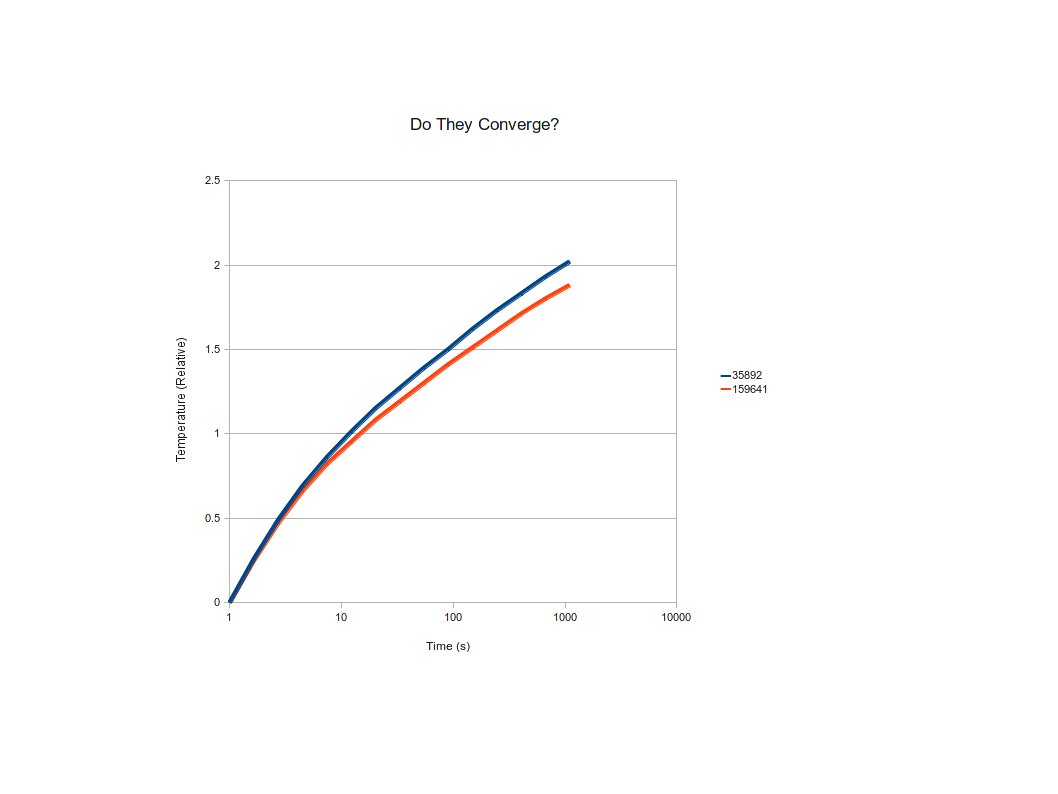
\includegraphics[width=0.6\textwidth]{fig/conv_curves.png}
\label{fig:conv_curves}
\caption{These two curves look similar enough, right?}
\end{figure}


\begin{table}[h]
\centering
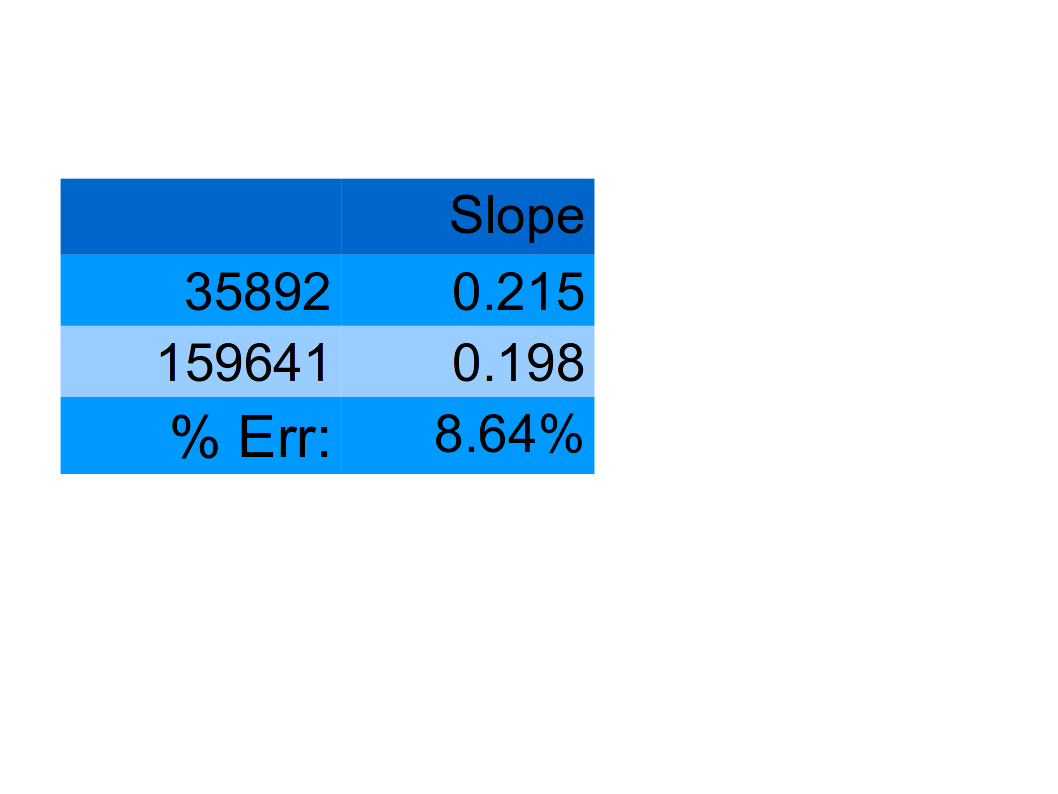
\includegraphics[width=0.6\textwidth]{fig/conv_kvals.png}
\label{tab:conv_kvals}
\caption{Despite the similarities in time/temperature curves, the resulting 
conductivity calculations differ by nearly 10 \%.}
\end{table}

\section{Benchtop Measurements}

The results of the benchtop measurements are mixed.

\begin{figure}[h]
\centering
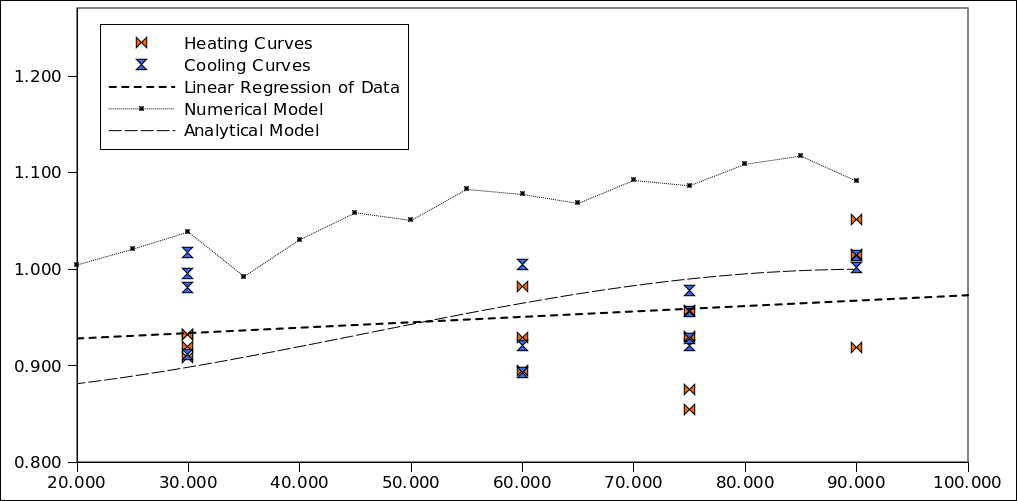
\includegraphics[width=0.9\textwidth]{fig/test_results.png}
\label{fig:test_results}
\caption{A comparison of the benchtop measurements with the numerical and
analytical predictions, given the calculated anisotropic thermal conductivity.}
\end{figure}

\begin{figure}[h]
\centering
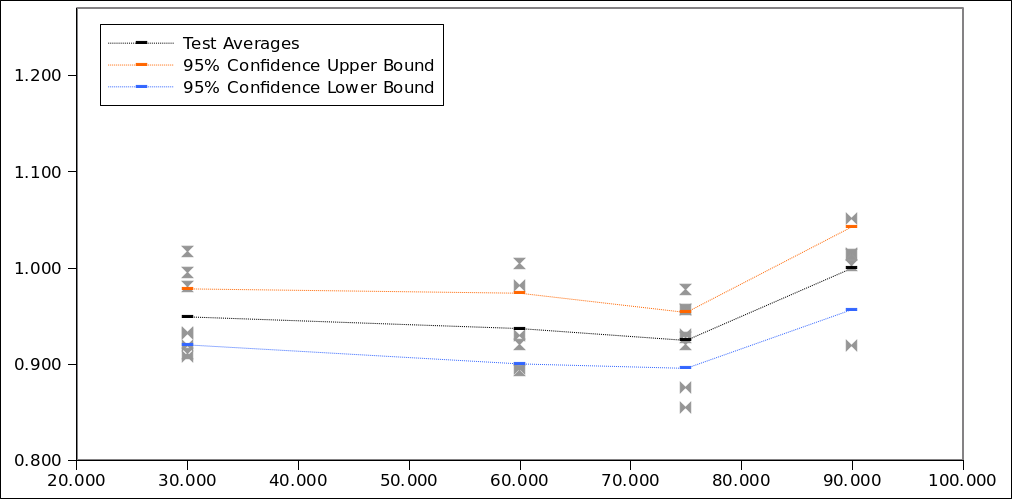
\includegraphics[width=0.9\textwidth]{fig/test_results_confidence.png}
\label{fig:test_confidence}
\caption{Upper and lower bounds of 90 \% confidence in measurements.}
\end{figure}

First, it may be seen that there is a significant amount of noise inherent in
the needle probe method, even accounting for obvious ``garbage measurements.''
This is likely due in part to the numerical derivative, but also in part due to
the method's sensitivity to errors in time measurement---that is, setting \(t_0\)
even half a second off may strongly influence the resulting measurement. Given
this noise, it is difficult to see which of the two models is more appropriate.

\marginpar{I saw this sensitivity from experience, but I should prove it 
to myself and the readers.}

Also given this noise and the relatively weak levels of anisotropy in the
sample, it would be difficult to deduce the degree of anisotropy of the sample
with this data and a curve fit alone, and probably even with more measurements.

However, it can be seen that, overall, the tests \emph{do} indicate anisotropy.
The general trends seen in the measurements do match the general trends seen in
the numerical and analytical models. This indicates that there may be hope in
refining this approach into a useful technique for measuring anisotropy.

\section{In-Situ Snow Measurements}

\begin{figure}[h]
\centering
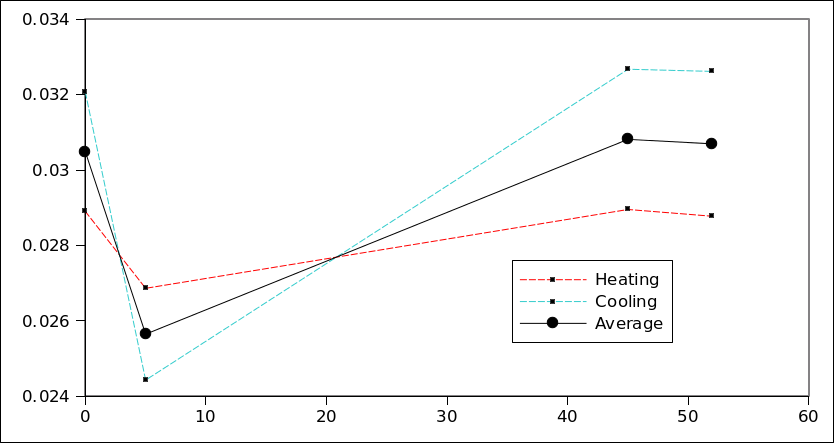
\includegraphics[width=0.9\textwidth]{fig/snow_meas.png}
\label{fig:test_results}
\caption{Even a limited amount of in-situ snow measurements show a degree of
anisotropy.}
\end{figure}

Due to the difficulty in taking snow measurements on top of the inherent noise
of the method, snow measurements resulted in being inconclusive. The 
measurements indicate anisotropy, as expected. However, the erratic nature of
the measurements suggests that the apparent trend could be as much operator
error as anything else. Either way, it indicates that, like the case of the
salt/sugar benchtop experiments, that levels of anisotropy appear relatively
weak, though probably detectable with enough measurements.
